
En la realización de nuestro trabajo, el de desarrollar aplicaciones, nos exponemos a
diferentes riesgos laborales. Algunos son muy comunes, como las caídas, y otros son más especificamos
del trabajo realizado, como algunos trastornos musculoesqueléticos. En este apartado vamos a analizar
los riesgos detectados en el trabajo del desarrollador, y propondremos acciones preventivas para
reducir ese riesgo.\\

\subsubsection{El puesto de trabajo}
El puesto de trabajo de un desarrollador suele tener los siguientes elementos:
\begin{itemize}
    \item Una mesa
    \item Una silla
    \item Un ordenador
    \item Teclado
    \item Monitor(es)
\end{itemize}
Todo esto suele estar ubicado en un espacio de oficina, o en casa en el caso de ser un
trabajo realizado en remoto en casa. Para evitar al máximo los riesgos laborales, deberemos 
tener en cuenta todos los elementos citados y diferentes factores ambientales como la temperatura o la iluminación.

\begin{figure}[H]
    \centering
    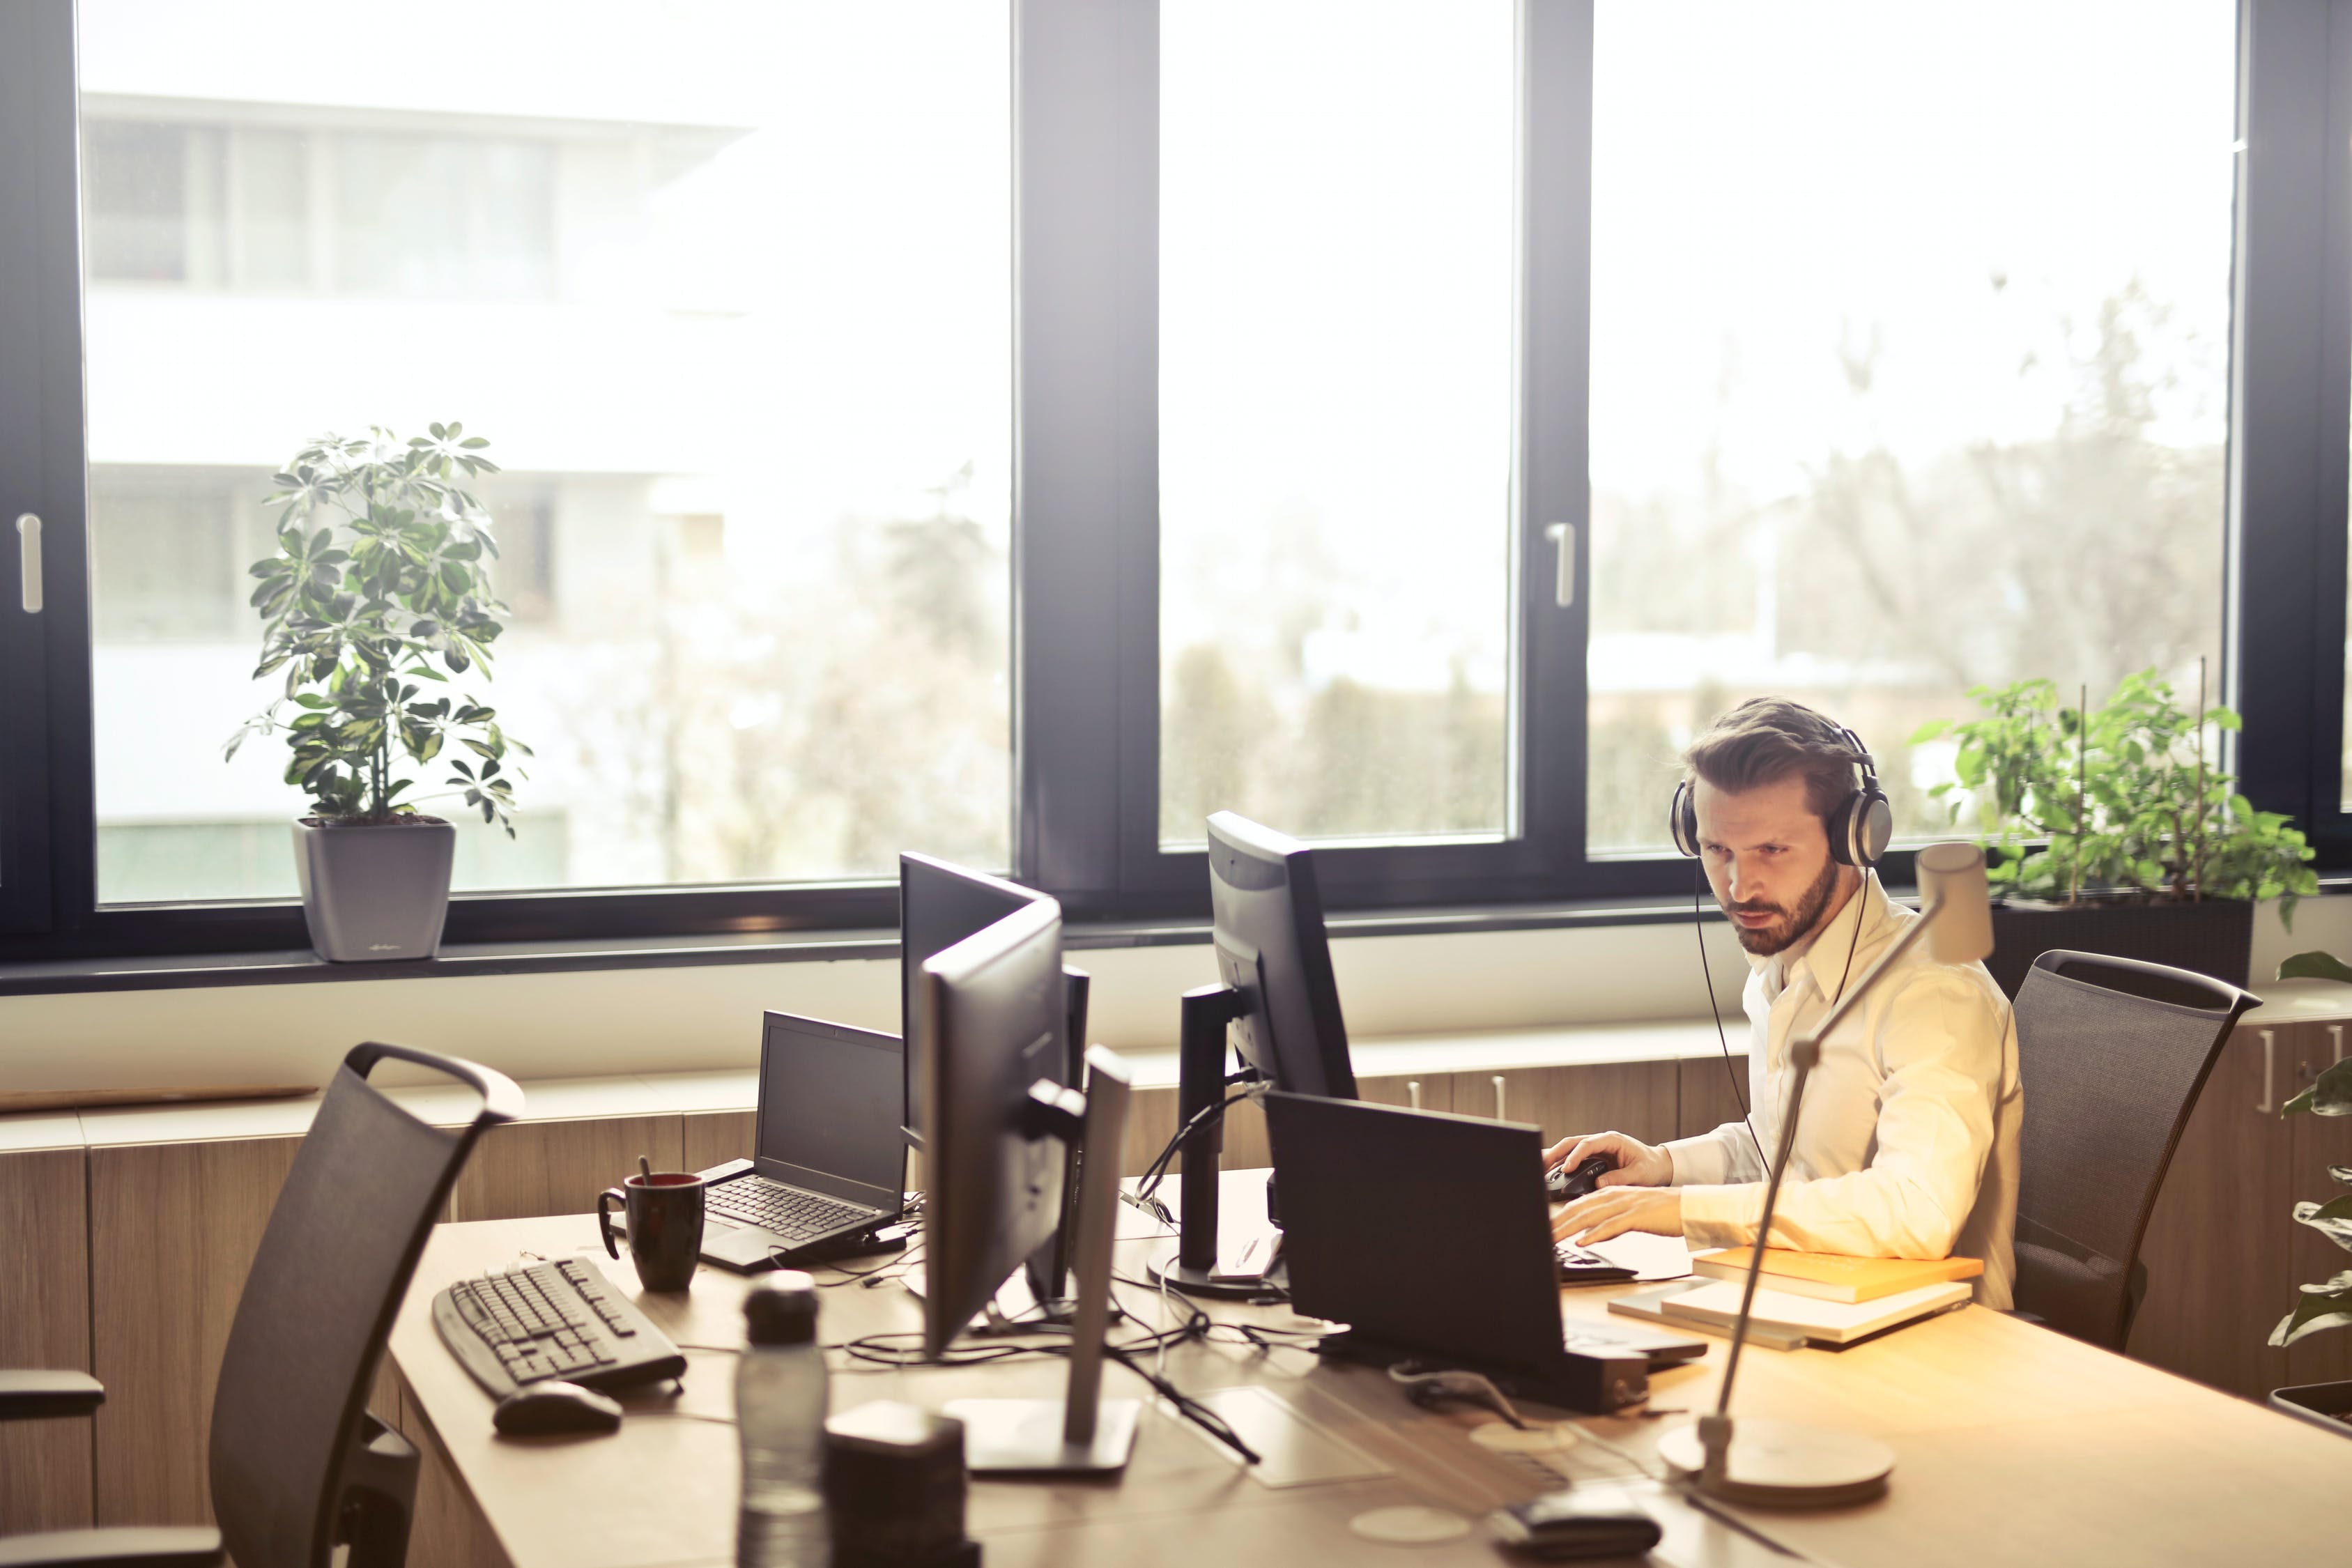
\includegraphics[width=1.0\textwidth]{Fol/oficina.jpeg}
    \caption{Ilustración de un puesto de trabajo de desarrollador}
    \caption*{\href{https://www.pexels.com/es-es/foto/hombre-con-auriculares-frente-al-monitor-de-la-computadora-845451/}{Fuente: https://www.pexels.com/es-es/}}
\end{figure}

\subsubsection{Riesgos Laborales}

En la siguiente imagen mostramos los riesgos más habituales en nuestro trabajo:

\begin{figure}[H]
    \centering
    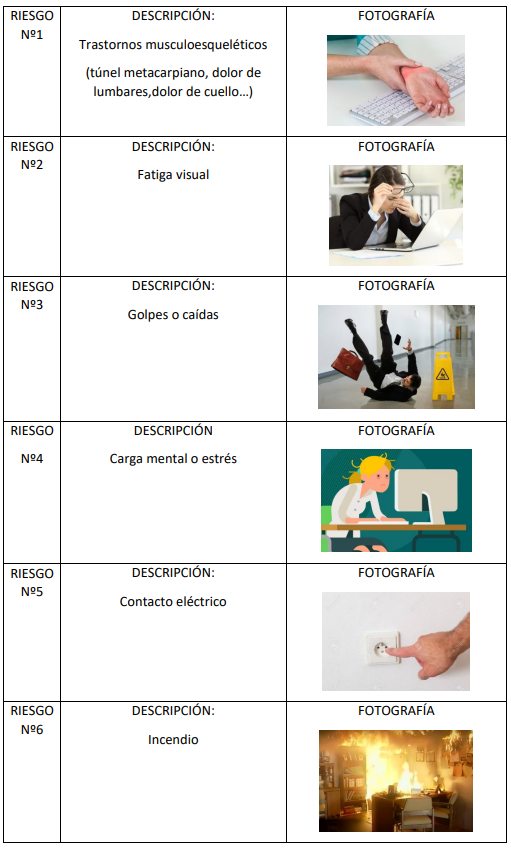
\includegraphics[width=1.0\textwidth]{Fol/tablaRiesgos.PNG}
    \caption{Tabla de riesgos laborales detectados.}
\end{figure}

\subsubsection{Evaluación de riesgos}
Para evaluar el nivel de riesgo que suponen los anteriores riesgos, se tiene en cuenta la probabilidad de que suceda
y las consecuencias del mismo. Basandonos en las pautas otorgadas por el \href{https://www.insst.es/documents/94886/96076/Evaluacion_riesgos.pdf/1371c8cb-7321-48c0-880b-611f6f380c1d?t=1526651610041}{\color{red}{INSST}},
hemos evaluado los riesgos de la siguiente manera: \\
\begin{itemize}
    \item Riesgo Nº1: Trastornos musculoesqueléticos: \begin{itemize}
              \item Probabilidad: Alta
              \item Consecuencias: Dañino
              \item Evaluación: Riesgo importante
          \end{itemize}
    \item Riesgo Nº2: Fatiga Visual: \begin{itemize}
              \item Probabilidad: Alta
              \item Consecuencias: Ligeramente dañino
              \item Evaluación: Riesgo moderado
          \end{itemize}
    \item Riesgo Nº3: Golpes o caídas: \begin{itemize}
              \item Probabilidad: Baja
              \item Consecuencias: Ligeramente dañino
              \item Evaluación: Riesgo trivial
          \end{itemize}
    \item Riesgo Nº4: Carga mental o estrés: \begin{itemize}
              \item Probabilidad: Alta
              \item Consecuencias: Ligeramente dañino - Extremadamente dañino
              \item Evaluación: Riesgo importante/Riesgo intolerable
          \end{itemize}
    \item Riesgo Nº5: Contacto eléctrico: \begin{itemize}
            \item Probabilidad: Baja
            \item Consecuencias: Extremadamente dañino
            \item Evaluación: Riesgo moderado
        \end{itemize}
    \item Riesgo Nº6: Incendio: \begin{itemize}
              \item Probabilidad: Baja
              \item Consecuencias: Extremadamente dañino
              \item Evaluación: Riesgo moderado
          \end{itemize}
\end{itemize}

\subsubsection{Medidas preventivas}
Para reducir en la medida de lo posible los anteriores riesgos, son necesarias algunas medidas preventivas.
Propondremos especificas para cada riesgo:\\
\paragraph*{Riesgo Nº1}
Para evitar los trastornos musculoesqueléticos más habituales (sindrome del túnel carpiano y dolor de lumbares), debemos
tener un espacio de trabajo ergonómico, es decir, adaptado al trabajador. La altura de la mesa debe ir ajustada al trabajador, y la
silla debería ser regulable y disponer de apoyo lumbar.
\begin{figure}[H]
    \centering
    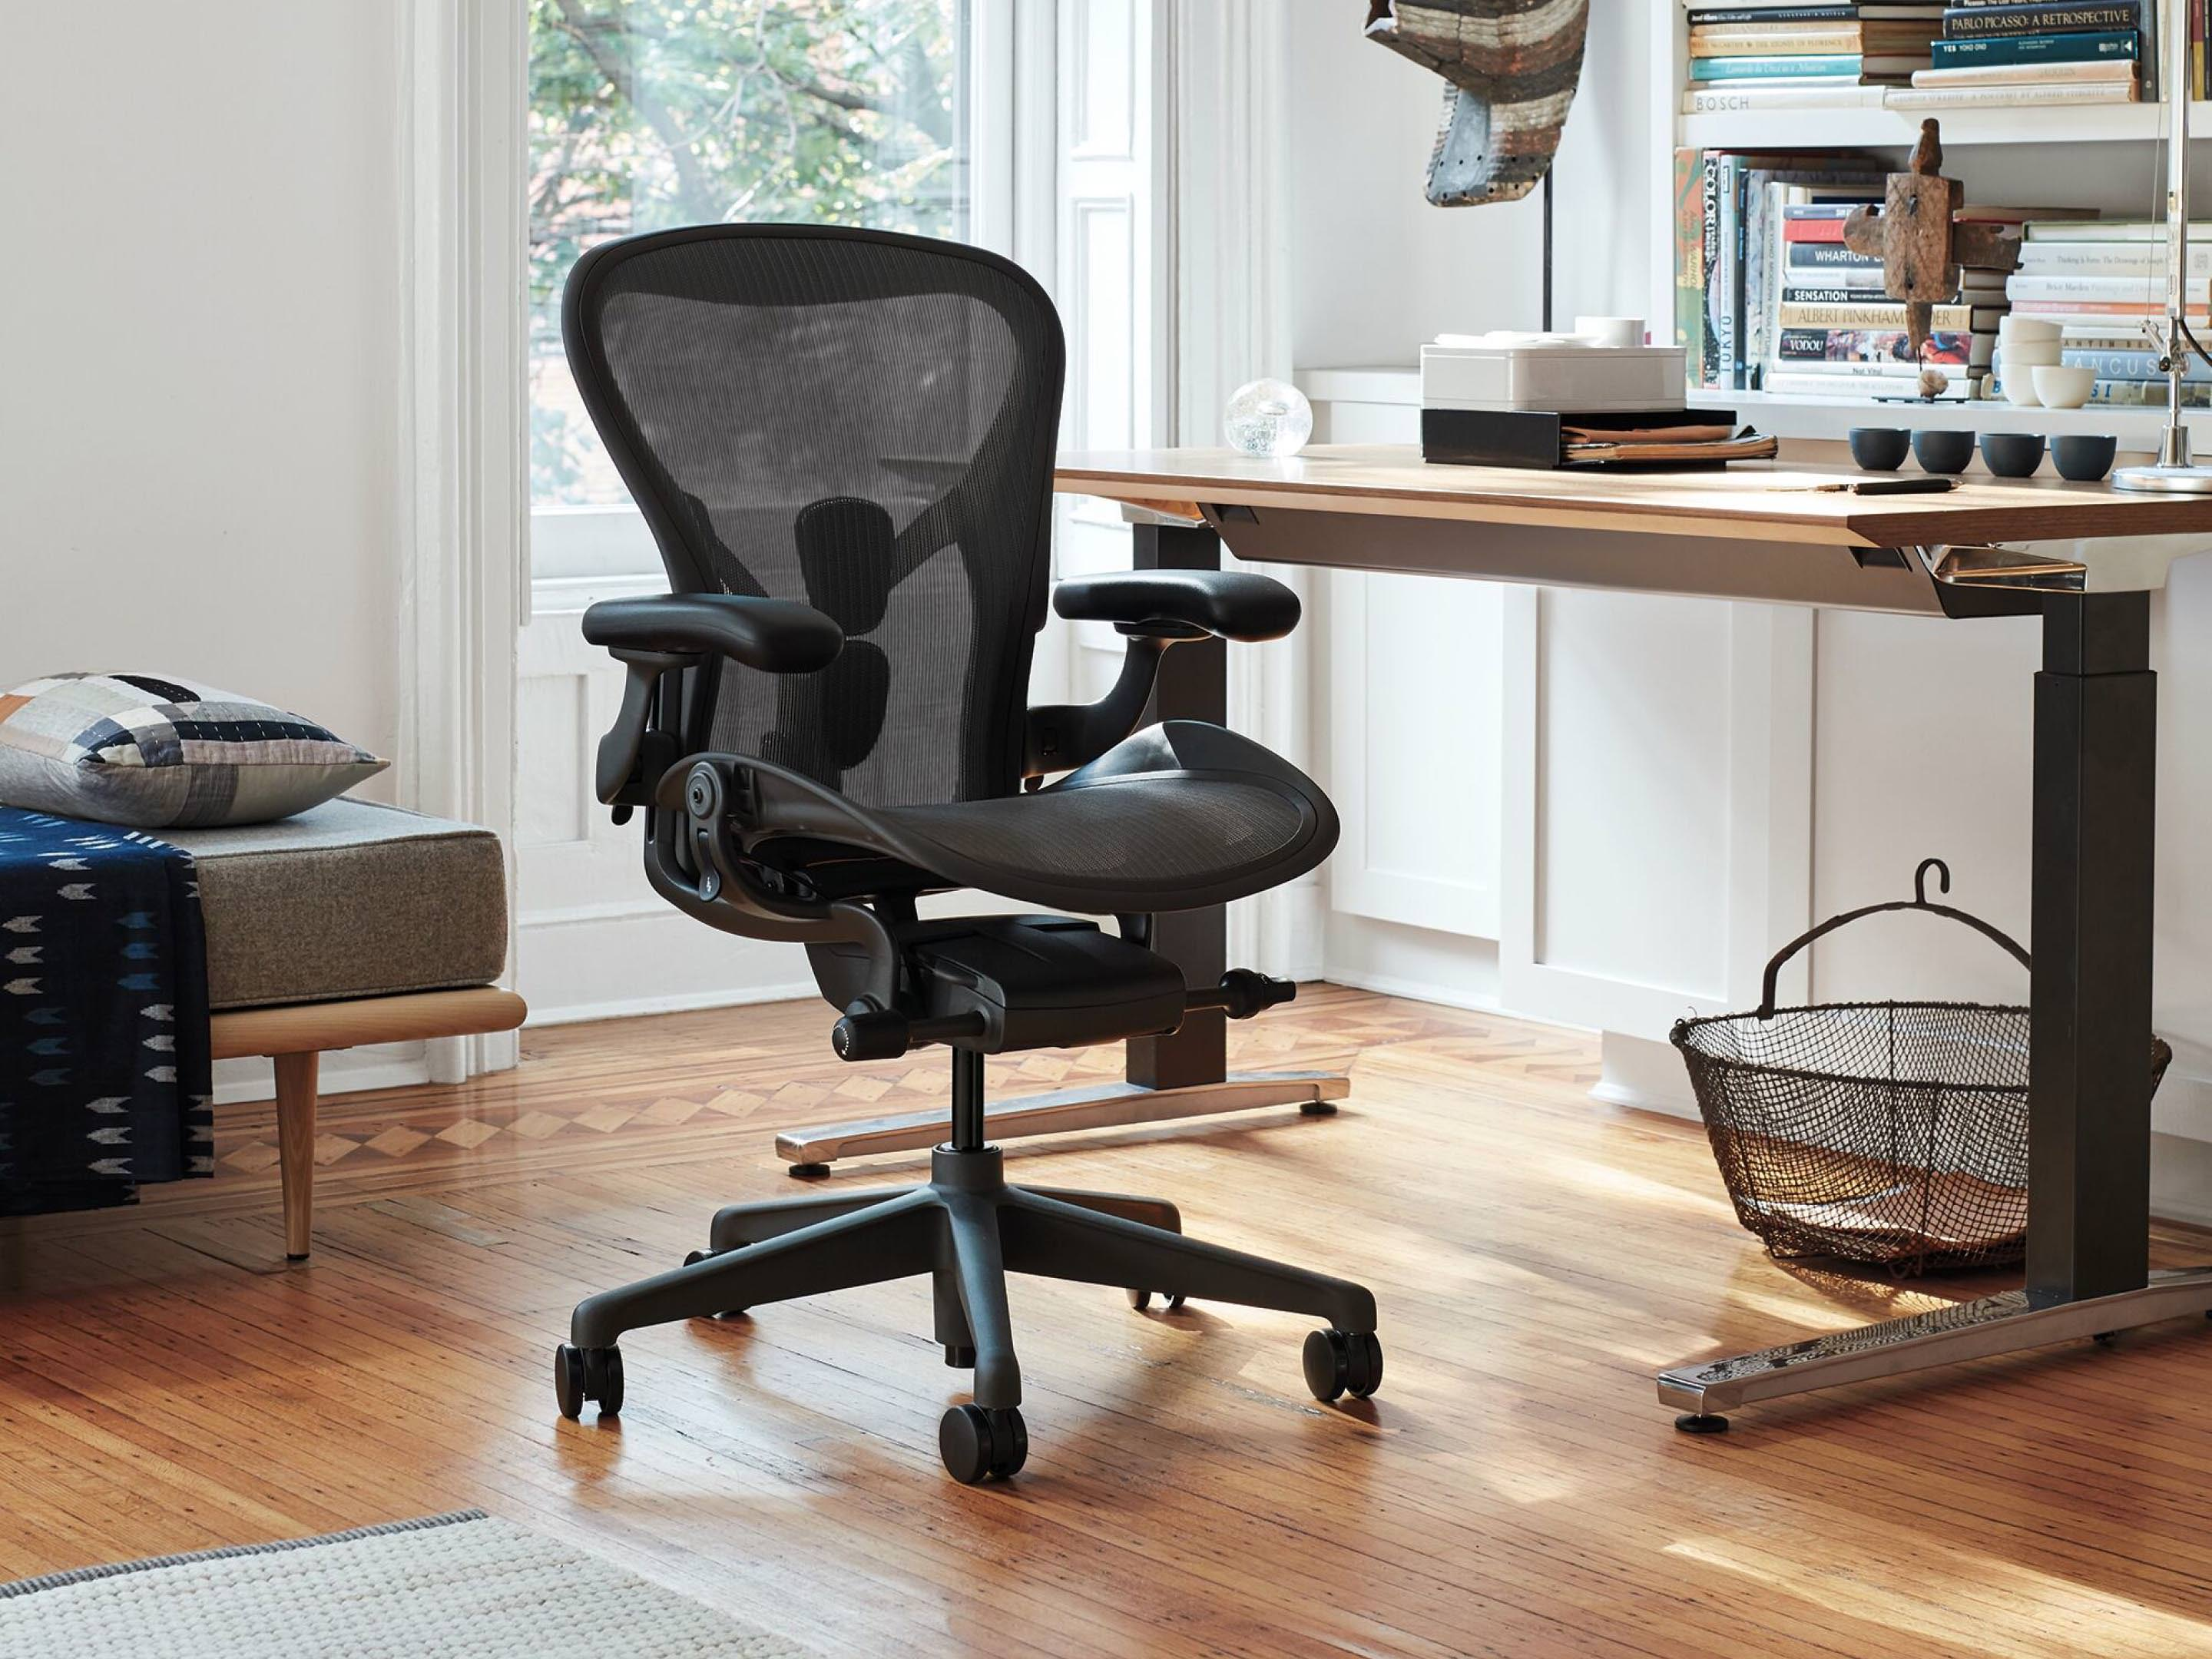
\includegraphics[width=1.0\textwidth]{Fol/silla.jpg}
    \caption{Ejemplo silla ergonómica}
    \caption*{\href{https://www.hermanmiller.com/es_mx/products/seating/office-chairs/aeron-chairs/}{Fuente: Herman Miller}}
\end{figure}

Los expertos en ergonomía suelen recomendar adoptar la siguiente postura a la hora de trabajar en un puesto como el nuestro:

\begin{figure}[H]
    \centering
    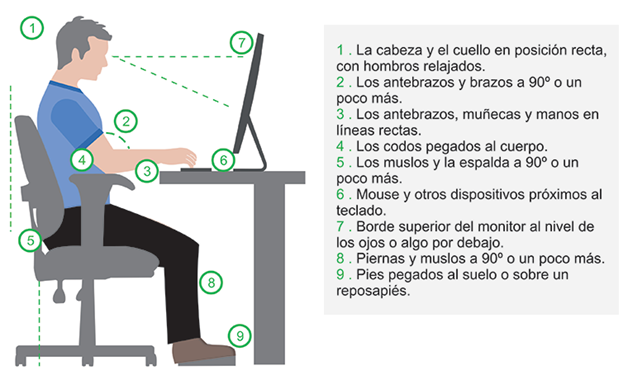
\includegraphics[width=1.0\textwidth]{Fol/posturaCorrecta.png}
    \caption{Postura correcta para trabajar con un ordenador}
\end{figure}

\paragraph*{Riesgo Nº2}
Para reducir el riesgo de fatiga visual, es importante tener una iluminación
homogénea del espacio de trabajo, además de un monitor calibrado y a una distancia
adecuada.\\
En el caso de una oficina, la iluminación mínima debería ser de 500 lux, utilizando la mayor cantidad de luz natural posible
\paragraph*{Riesgo Nº3}
Para evitar caídas o golpes al mismo nivel, debemos asegurar que el suelo esté seco y
no sea una superficie resbaladiza. \\
En caso de haber escaleras, también debemos colocar barandillas y elementos antideslizantes, y asegurarnos que los peldaños tienen una
huella entre 23-36cm y una contrahuella entre 13-20cm.
\begin{figure}[H]
    \centering
    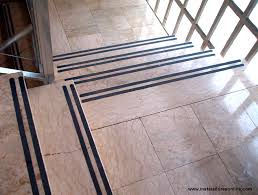
\includegraphics[width=1.0\textwidth]{Fol/elemAntides.jpg}
    \caption{Elementos antideslizantes en escaleras}
    \caption*{\href{http://www.instaladoresonline.com/cintas_antideslizantes_safety_walk.html}{Fuente: https://www.instaladoresonline.com/}}
\end{figure}
\paragraph*{Riesgo Nº4}
Para evitar el estrés y una carga mental excesiva, es importante distribuir bien el trabajo 
y establecer plazos realistas. Además de ello, es importante fomentar un buen ambiente laboral para
evitar que en posibles fases de carga alta el estrés se agrave. \\ 
Y lo más importante, es primordial establecer y respetar periodos de descanso legales y necesarios. 
\paragraph*{Riesgo Nº5}
Para evitar contactos eléctricos, debemos tener todos los ordenadores en óptimas
condiciones. Un chasis en mal estado podría conducir la corriente y provocar
calambres. Además de ello, deberíamos minimizar la necesidad de los empleados de
andar enchufando y desenchufando aparatos, aportándoles un espacio de trabajo
propio estático.
\paragraph*{Riesgo Nº6}
Como en todos los edificios, para evitar los incendios es importante que todo el
cableado eléctrico (y ordenadores) esté en buenas condiciones, además de tener
extintores colocados en los pasillos y habitaciones.
